\documentclass[11pt,a4paper]{article}

\usepackage[T1]{fontenc}
\usepackage[utf8]{inputenc}
\usepackage[brazilian]{babel}
\usepackage{lmodern}
\usepackage{microtype}
\usepackage[margin=2.2cm]{geometry}
\usepackage{graphicx}
\usepackage{booktabs}
\usepackage{tabularx}
\usepackage{float}
\usepackage{caption}
\usepackage{xcolor}
\usepackage{enumitem}
\usepackage[hidelinks]{hyperref}

\graphicspath{{figuras/}}
\captionsetup{font=small,labelfont=bf}
\setlist{itemsep=2pt,topsep=4pt}
\renewcommand{\arraystretch}{1.2}
\emergencystretch=3em

% Marca tudo o que ainda depende de captura ou medição real.
% Antes da entrega não pode sobrar nenhuma ocorrência no PDF.
\newcommand{\pendente}[1]{\textcolor{red}{\textbf{[PENDENTE: #1]}}}

\newcommand{\cod}[1]{\texttt{#1}}

\title{Servidor HTTP/1.1 sobre Sockets TCP\\[4pt]
\large Laboratório de Redes de Computadores --- Trabalho 1}
\author{Anthony Antonelli \and Leonardo Fagundes \and Lucas Simão \and Samuel Bitdinger}
\date{Testes realizados em 3 de outubro de 2026}

\begin{document}
\maketitle

\section{Arquitetura e concorrência}

O servidor foi escrito em Java e usa apenas \cod{java.net.ServerSocket} e
\cod{java.net.Socket}. Nenhuma biblioteca HTTP de servidor é utilizada: a
leitura da requisição e a montagem da resposta são feitas pelo nosso código.
As responsabilidades estão divididas em seis classes:

\begin{itemize}
  \item \cod{ServerConfig} lê e valida os argumentos \cod{-{}-port},
  \cod{-{}-root}, \cod{-{}-idle-timeout} e \cod{-{}-workers}.
  \item \cod{ServerMain} abre o socket em \cod{0.0.0.0}, aceita conexões e
  entrega cada uma a um \emph{pool} fixo de threads.
  \item \cod{HttpRequestReader} acumula os bytes recebidos em um buffer até
  encontrar \cod{\textbackslash r\textbackslash n\textbackslash
  r\textbackslash n}. O que vier depois desse marcador fica guardado para a
  requisição seguinte, já que o TCP entrega um fluxo de bytes e uma leitura
  pode trazer meia requisição ou uma requisição e o começo da próxima.
  \item \cod{StaticFileService} decodifica o percent-encoding, normaliza o
  caminho e só abre o arquivo se o caminho real estiver dentro da raiz.
  \item \cod{HttpResponseWriter} escreve a linha de status e os cabeçalhos
  \cod{Date} (IMF-fixdate em GMT), \cod{Server}, \cod{Content-Type} e
  \cod{Content-Length}. No \cod{GET} o corpo sai em blocos de até 16\,KiB; no
  \cod{HEAD} os cabeçalhos são os mesmos e o corpo não é enviado.
  \item \cod{HttpConnectionHandler} atende requisições em sequência na mesma
  conexão até receber \cod{Connection: close}, estourar o timeout de
  ociosidade ou o cliente fechar o socket.
\end{itemize}

\paragraph{Estratégia de concorrência.} Adotamos uma thread por conexão,
tiradas de um \emph{pool} de tamanho fixo (padrão: o maior entre 4 e o número
de CPUs). O modelo é bloqueante, então o código de cada conexão é linear e
fácil de explicar: lê, processa, responde, repete. O \emph{pool} limita o
número de threads, o que impede que uma rajada de conexões crie threads sem
controle. Uma requisição lenta ocupa só a própria thread e as outras conexões
seguem sendo atendidas enquanto houver thread livre. Quando todas estão
ocupadas, as novas conexões esperam na fila do executor.

Duas limitações conhecidas: a fila do executor não tem tamanho máximo, e o
timeout vale para leitura, não para escrita. Um cliente que pare de ler a
resposta pode segurar uma thread.

\paragraph{Configuração usada nos testes.} Porta 8080, raiz \cod{./www},
timeout de ociosidade de 5000\,ms. O servidor rodou em um MacBook (macOS) e o cliente principal em uma máquina Windows
da mesma rede local, com \cod{curl.exe} no PowerShell. Os endereços IP foram
omitidos do texto e aparecem borrados nas figuras.

\section{Conformidade HTTP}

{\sloppy A Tabela~\ref{tab:conformidade} traz, para cada código obrigatório, o comando
executado no cliente e a resposta recebida. Em todos os casos a base é
\cod{http://<servidor>:8080}. As Figuras~\ref{fig:get} a~\ref{fig:405}
mostram as saídas obtidas.\par}

\begin{table}[H]
\centering
\small
\begin{tabularx}{\textwidth}{@{}l>{\raggedright\arraybackslash}X>{\raggedright\arraybackslash}X@{}}
\toprule
\textbf{Código} & \textbf{Requisição} & \textbf{Resposta obtida} \\
\midrule
200 (GET) & \cod{curl.exe -{}-http1.1 -i "\$BASE/index.html"} &
\cod{HTTP/1.1 200 OK}, \cod{Content-Length: 2294}, \cod{Content-Type:
text/html; charset=utf-8}, corpo com o HTML \\
200 (HEAD) & \cod{curl.exe -{}-http1.1 -I "\$BASE/index.html"} &
\cod{HTTP/1.1 200 OK}, mesmos cabeçalhos do GET (\cod{Content-Length: 2294}),
sem corpo \\
400 & \cod{curl.exe -{}-http1.1 -i -{}-request-target '/ alvo-invalido'
"\$BASE/"} & \cod{HTTP/1.1 400 Bad Request}, \cod{Content-Length: 17},
\cod{Connection: close} \\
403 & \cod{curl.exe -{}-http1.1 -{}-path-as-is "\$BASE/../../etc/passwd"} &
corpo \cod{403 Forbidden} (ver Seção~\ref{sec:seguranca}) \\
404 & \cod{curl.exe -{}-http1.1 -i "\$BASE/aaa.html"} &
\cod{HTTP/1.1 404 Not Found}, \cod{Content-Length: 15} \\
405 & \cod{curl.exe -{}-http1.1 -i -X POST "\$BASE/index.html"} &
\cod{HTTP/1.1 405 Method Not Allowed}, \cod{Content-Length: 24},
\cod{Allow: GET, HEAD} \\
\bottomrule
\end{tabularx}
\caption{Códigos de status obrigatórios, requisição e resposta.}
\label{tab:conformidade}
\end{table}

Todas as respostas trazem \cod{Date} em GMT e o cabeçalho \cod{Server}
com o valor \cod{Grupo-Redes-HTTP1.1}. O \cod{Content-Length} de 2294 bytes é o tamanho
exato de \cod{www/index.html}, e o valor é o mesmo no GET e no HEAD. As
respostas de erro têm \cod{Content-Length} igual ao tamanho da mensagem
curta enviada no corpo. O 400 fecha a conexão porque, depois de uma linha de
requisição inválida, o servidor não tem como saber onde começa a próxima.

\begin{figure}[H]
\centering
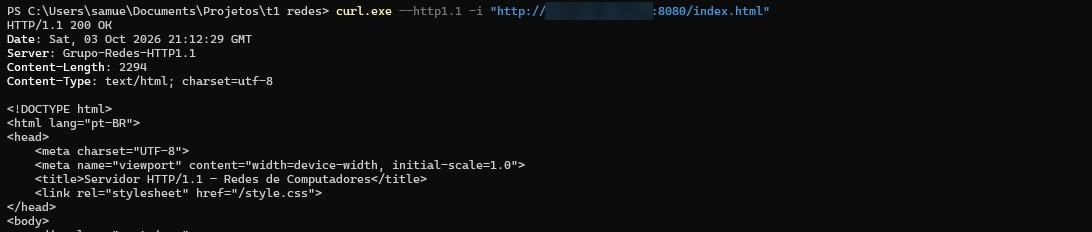
\includegraphics[width=0.95\textwidth]{curl-get-200}
\caption{GET de \cod{index.html}: 200 OK com os cabeçalhos e o começo do corpo.}
\label{fig:get}
\end{figure}

\begin{figure}[H]
\centering
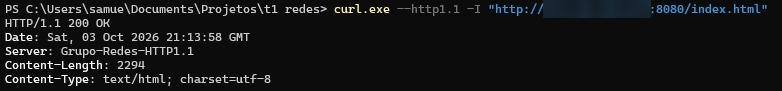
\includegraphics[width=0.85\textwidth]{curl-head-200}\\[6pt]
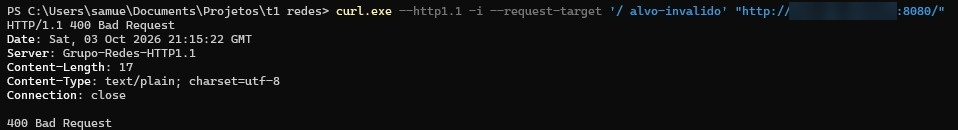
\includegraphics[width=0.95\textwidth]{curl-400-bad-request}\\[6pt]
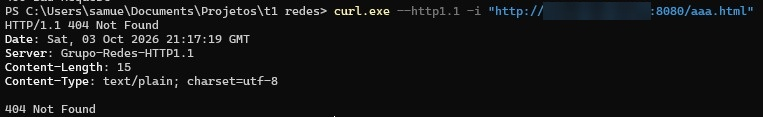
\includegraphics[width=0.85\textwidth]{curl-404-not-found}\\[6pt]
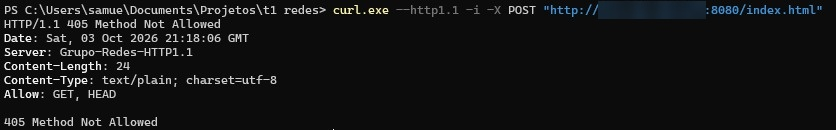
\includegraphics[width=0.9\textwidth]{curl-405-post}
\caption{De cima para baixo: HEAD (200, sem corpo), linha de requisição
inválida (400), arquivo inexistente (404) e POST (405 com \cod{Allow}).}
\label{fig:405}
\end{figure}

\section{Segurança: travessia de diretório}
\label{sec:seguranca}

O \cod{StaticFileService} decodifica o caminho, resolve os \cod{..} e
compara o caminho real resultante com a raiz configurada. Se o resultado
sair da raiz, a resposta é 403, exista o arquivo ou não. A opção
\cod{-{}-path-as-is} é necessária porque, sem ela, o próprio curl remove os
\cod{../} antes de enviar.

\begin{table}[H]
\centering
\small
\begin{tabularx}{\textwidth}{@{}l>{\raggedright\arraybackslash}X l@{}}
\toprule
\textbf{Tentativa} & \textbf{Caminho enviado} & \textbf{Resposta} \\
\midrule
\cod{../} literal & \cod{/../../etc/passwd} & \cod{403 Forbidden} \\
\cod{../} literal & \cod{/../../outside.txt} & \cod{403 Forbidden} \\
Percent-encoding & \cod{/\%2e\%2e/\%2e\%2e/outside.txt} & \cod{403 Forbidden} \\
Prefixo válido + encoding & \cod{/safe/\%2e\%2e/\%2e\%2e/outside.txt} & \cod{403 Forbidden} \\
\bottomrule
\end{tabularx}
\caption{Tentativas de travessia rejeitadas pelo servidor.}
\label{tab:travessia}
\end{table}

\begin{figure}[H]
\centering
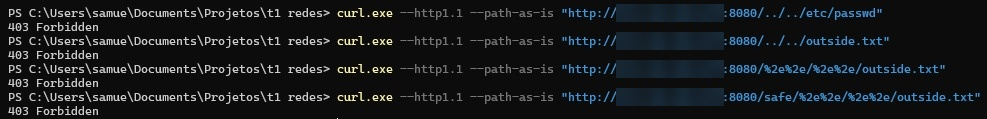
\includegraphics[width=\textwidth]{curl-403-travessia}
\caption{As quatro tentativas, feitas a partir da máquina cliente. Os
comandos foram executados sem \cod{-i}, por isso aparece só o corpo da
resposta.}
\label{fig:travessia}
\end{figure}

\section{Transação GET completa}

A transação analisada é a primeira conexão da captura \cod{capturas/c1.pcapng},
feita no servidor com o filtro \cod{tcp.port == 8080}. O cliente Windows
executou \cod{curl.exe -{}-http1.1 -H 'Connection: close' "\$BASE/index.html"};
a Figura~\ref{fig:close} mostra a mesma requisição vista pelo terminal. A
Tabela~\ref{tab:transacao} lista os quadros, com o tempo contado a partir do
SYN.

\begin{figure}[H]
\centering
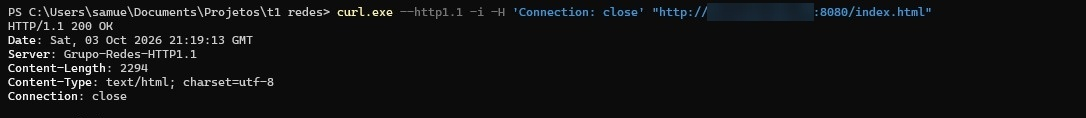
\includegraphics[width=0.95\textwidth]{curl-get-connection-close}
\caption{GET com \cod{Connection: close}, visto pelo cliente (início da saída).}
\label{fig:close}
\end{figure}

\begin{table}[H]
\centering
\small
\begin{tabular}{@{}rrllrl@{}}
\toprule
\textbf{Quadro} & \textbf{t (ms)} & \textbf{Sentido} & \textbf{Flags} &
\textbf{Bytes} & \textbf{Conteúdo} \\
\midrule
1 & 0,000 & cliente $\to$ servidor & SYN & 66 & abertura \\
2 & 0,351 & servidor $\to$ cliente & SYN, ACK & 66 & abertura \\
3 & 3,717 & cliente $\to$ servidor & ACK & 60 & fim do handshake \\
\midrule
4 & 3,719 & cliente $\to$ servidor & PSH, ACK & 167 & \cod{GET /index.html HTTP/1.1} (113 bytes) \\
5 & 3,808 & servidor $\to$ cliente & ACK & 54 & confirma a requisição \\
6 & 6,030 & servidor $\to$ cliente & PSH, ACK & 220 & \cod{HTTP/1.1 200 OK} e cabeçalhos (166 bytes) \\
7 & 6,159 & servidor $\to$ cliente & ACK & 1514 & corpo, 1460 bytes \\
8 & 6,166 & servidor $\to$ cliente & PSH, ACK & 888 & corpo, 834 bytes \\
\midrule
9 & 6,272 & servidor $\to$ cliente & FIN, ACK & 54 & servidor encerra \\
10 & 10,026 & cliente $\to$ servidor & ACK & 60 & confirma os dados e o FIN \\
11 & 10,027 & cliente $\to$ servidor & FIN, ACK & 60 & cliente encerra \\
13 & 10,133 & servidor $\to$ cliente & ACK & 54 & confirma o FIN \\
\bottomrule
\end{tabular}
\caption{Quadros da primeira conexão de \cod{c1.pcapng}: handshake (1 a 3),
requisição e resposta (4 a 8) e encerramento (9 a 13). O quadro 12 é o SYN da
conexão seguinte.}
\label{tab:transacao}
\end{table}

O corpo de 2294 bytes não cabe em um segmento (MSS de 1460 bytes) e sai em
dois, 1460 + 834. Como a requisição pediu \cod{Connection: close}, é o servidor
que manda o primeiro FIN, logo depois do último segmento do corpo.

\section{Atendimento simultâneo}

O teste está em \cod{capturas/concorrencia.pcapng} e usa duas máquinas
clientes, com IPs diferentes. O cliente A abre uma conexão e envia só o começo
da requisição (a linha \cod{GET} e o cabeçalho \cod{Host}, sem a linha em
branco final). A thread que atende A fica bloqueada esperando o resto.
Enquanto isso, o cliente B faz um GET completo.

\begin{table}[H]
\centering
\small
\begin{tabular}{@{}rlll@{}}
\toprule
\textbf{t (s)} & \textbf{Cliente} & \textbf{Quadros} & \textbf{Evento} \\
\midrule
0,000 & A & 1 a 4 & handshake \\
0,395 & A & 5 & requisição parcial, 49 bytes, sem \cod{\textbackslash r\textbackslash n\textbackslash r\textbackslash n} \\
4,921 & B & 9 a 11 & handshake \\
4,939 & B & 13 & \cod{GET /index.html} completo \\
4,967 & B & 15 a 17 & \cod{200 OK} e corpo (2294 bytes) \\
4,982 & B & 19 a 22 & encerramento \\
10,402 & A & 23 & resto da requisição (\cod{Connection: close} e linha em branco) \\
10,404 & A & 25 a 27 & \cod{200 OK} e corpo (2294 bytes) \\
10,414 & A & 28 a 32 & encerramento \\
\bottomrule
\end{tabular}
\caption{Linha do tempo de \cod{concorrencia.pcapng}. A conexão de A fica
aberta de 0 a 10,4\,s; B é atendido por inteiro nesse intervalo.}
\label{tab:concorrencia}
\end{table}

B recebeu a resposta 28\,ms depois de enviar o GET, com a conexão de A ainda
aberta e incompleta. Um servidor de uma thread só ficaria parado na leitura de
A e B esperaria mais de 5\,s. Depois, A completou a requisição e também recebeu
200. Para que a requisição parcial de A não expirasse durante os 10\,s do
teste, o servidor foi iniciado com \cod{-{}-idle-timeout} maior que o padrão.

\section{RTT entre as máquinas}

O RTT foi medido com dez pacotes ICMP entre as duas máquinas usadas nos
testes (Figura~\ref{fig:ping}). Não houve perda.

\begin{table}[H]
\centering
\small
\begin{tabular}{@{}cccc@{}}
\toprule
\textbf{Mínimo} & \textbf{Médio} & \textbf{Máximo} & \textbf{Desvio padrão} \\
\midrule
2,756 ms & \textbf{3,918 ms} & 7,730 ms & 1,907 ms \\
\bottomrule
\end{tabular}
\caption{RTT medido com \cod{ping -c 10 <IP>}.}
\end{table}

\begin{figure}[H]
\centering
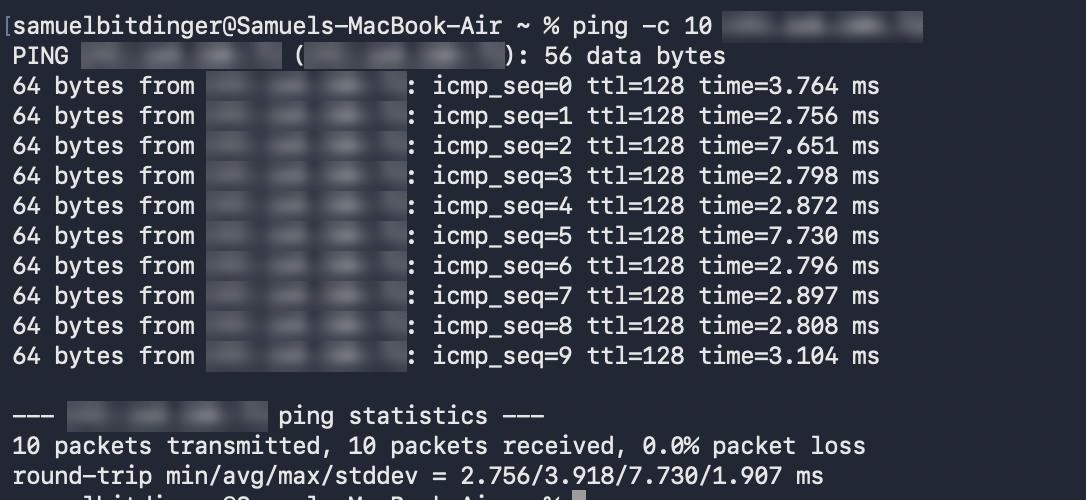
\includegraphics[width=0.7\textwidth]{ping-rtt}
\caption{Saída do \cod{ping} entre as máquinas do teste.}
\label{fig:ping}
\end{figure}

\section{Comparação C1 $\times$ C2}

Os dois cenários fazem dez GETs sequenciais de \cod{/index.html} (2294 bytes)
com os scripts \cod{measure-c1.sh} e \cod{measure-c2.sh}. Em C1 cada
requisição leva \cod{Connection: close} e abre uma conexão nova; em C2 as dez
requisições usam a mesma conexão. As capturas são \cod{capturas/c1.pcapng} e
\cod{capturas/c2.pcapng}, feitas no servidor. Os bytes são a soma do tamanho
dos quadros (\cod{frame.len}) nos dois sentidos, e o tempo vai do primeiro SYN
ao último ACK do encerramento.

\begin{table}[H]
\centering
\small
\begin{tabular}{@{}lccc@{}}
\toprule
\textbf{Métrica} & \textbf{C1} & \textbf{C2} & \textbf{Economia} \\
\midrule
Handshakes TCP completos & 10 & 1 & --- \\
Total de pacotes & 120 & 67 & 44,2\,\% \\
Bytes totais & 32\,630 & 29\,070 & 10,9\,\% \\
Tempo total (ms) & 105,6 & 64,5 & 39,0\,\% \\
\bottomrule
\end{tabular}
\caption{C1 (conexão nova por requisição) e C2 (conexão persistente).
Economia $= 100 \times (\mathrm{C1} - \mathrm{C2}) / \mathrm{C1}$.}
\label{tab:c1c2}
\end{table}

A economia de bytes é bem menor que a de pacotes porque os pacotes poupados
são de controle, com 54 a 66 bytes cada, enquanto o grosso dos bytes é o
conteúdo, igual nos dois cenários (dez vezes o mesmo arquivo). Não houve
retransmissão nem RST em nenhuma das capturas.

\section{Overhead de abertura e encerramento em C1}

As dez conexões de C1 são idênticas: 12 pacotes e 3263 bytes cada. Sete
desses pacotes não carregam dado nenhum e servem só para abrir e fechar a
conexão.

\begin{table}[H]
\centering
\small
\begin{tabular}{@{}lccc@{}}
\toprule
\textbf{Etapa} & \textbf{Por conexão} & \textbf{Pacotes} & \textbf{Bytes} \\
\midrule
Abertura (SYN, SYN/ACK, ACK) & 3 pacotes, 192 bytes & 30 & 1920 \\
Encerramento (FIN, ACK, FIN, ACK) & 4 pacotes, 228 bytes & 40 & 2280 \\
\midrule
Total & 7 pacotes, 420 bytes & 70 & 4200 \\
\bottomrule
\end{tabular}
\caption{Pacotes e bytes de controle de conexão em C1. As duas últimas colunas somam as dez conexões.}
\label{tab:overhead}
\end{table}

Abrir e fechar conexões consome 70 dos 120 pacotes de C1 (58,3\,\%) e 4200
dos 32\,630 bytes (12,9\,\%). Uma ressalva na contagem: o ACK do cliente no
encerramento (quadro 10 da Tabela~\ref{tab:transacao}) confirma ao mesmo tempo
os últimos dados e o FIN do servidor. Contamos esse pacote como encerramento.
Em C2 o cliente confirma cada resposta com um ACK separado, e isso explica a
diferença entre os cenários:

\begin{itemize}
  \item Pacotes: $9 \times 7 = 63$ de controle a menos, e 10 ACKs de dados a
  mais em C2. $63 - 10 = 53 = 120 - 67$.
  \item Bytes: $9 \times 420 = 3780$ de controle a menos, mais 380 bytes do
  cabeçalho \cod{Connection: close} (19 bytes na requisição e 19 na resposta,
  dez vezes), menos 600 bytes dos 10 ACKs. $3780 + 380 - 600 = 3560 =
  32\,630 - 29\,070$.
\end{itemize}

\section{Análise em função do RTT}

Cada conexão nova custa um RTT antes que a requisição possa sair: o cliente
envia o SYN, espera o SYN/ACK e só então manda o ACK e o GET. Na
Tabela~\ref{tab:transacao} isso aparece entre os quadros 2 e 3. A troca
requisição/resposta custa mais um RTT, e esse custo existe nos dois cenários.
C1 faz dez handshakes e C2 faz um, então C1 gasta nove RTTs a mais.

O encerramento não acrescenta espera. Na captura, o cliente manda o FIN de uma
conexão e o SYN da seguinte no mesmo instante (quadros 11 e 12, com 2\,$\mu$s de
diferença), sem aguardar o último ACK.

\begin{table}[H]
\centering
\small
\begin{tabular}{@{}lc@{}}
\toprule
Diferença medida, $t_{C1} - t_{C2}$ & 41,2 ms \\
Previsão com o RTT do ping, $9 \times 3{,}918$ ms & 35,3 ms \\
RTT médio dos dez handshakes de C1 (SYN/ACK até o ACK) & 4,484 ms \\
Previsão com o RTT dos handshakes, $9 \times 4{,}484$ ms & 40,4 ms \\
\bottomrule
\end{tabular}
\caption{Diferença de tempo entre os cenários e previsão do modelo.}
\end{table}

A diferença medida equivale a 10,5 RTTs do ping, contra os 9 previstos. O
motivo é que o RTT durante o teste foi maior que o do ping: medido na própria
captura, pelo intervalo entre o SYN/ACK do servidor e o ACK do cliente, ele
ficou entre 3,4 e 5,5\,ms, com média de 4,484\,ms. Com esse valor, nove
handshakes dão 40,4\,ms, a 0,8\,ms do medido.

Essa concordância tem uma coincidência por trás. Olhando o intervalo entre
GETs consecutivos, C1 leva em média 10,66\,ms por requisição e C2 leva
4,62\,ms (da segunda requisição em diante). A diferença, 6,0\,ms, é um RTT de
handshake mais cerca de 1,5\,ms, que vêm do tempo de resposta do servidor
(cerca de 1,0\,ms em C1 e 0,6\,ms em C2, porque cada conexão nova passa pelo
\cod{accept} e pela fila do \emph{pool}) e do trabalho do cliente para criar
outro socket. Em sentido contrário, a primeira requisição de C2 foi lenta:
14,0\,ms, com 6,5\,ms só para o servidor começar a responder, contra cerca
de 0,6\,ms nas seguintes. A captura não mostra a causa; o servidor estava
parado havia alguns minutos. Os dois efeitos quase se cancelam no total.

\section{Conclusão}

Com dez requisições e RTT em torno de 4\,ms, a conexão persistente usou 44\,\%
menos pacotes, 11\,\% menos bytes e terminou 41\,ms antes. Quase todo esse
tempo vem dos nove handshakes que C2 não faz.

O ganho da persistência depende de dois fatores: quantas conexões ela evita e
quanto custa cada uma. O custo de cada conexão evitada é de um RTT, então o
tempo poupado é aproximadamente $(N - 1) \times \mathrm{RTT}$ para $N$
requisições. Na nossa rede local isso deu 41\,ms. Em um enlace com RTT de
100\,ms, como um acesso intercontinental ou uma rede móvel congestionada, os
mesmos nove handshakes custariam cerca de 900\,ms, enquanto o tempo de
transferir os 2294 bytes mudaria pouco. Uma página com dezenas de recursos
pequenos aumenta $N$ e tem o mesmo efeito. O ganho seria maior que o medido,
portanto, em redes de RTT alto e com muitas requisições curtas para o mesmo
servidor. Com HTTPS a diferença cresceria ainda mais, porque cada conexão nova
também paga o handshake do TLS.

\end{document}
